\documentclass[5p]{elsarticle}
\usepackage{natbib}
\usepackage{url}
\begin{document}
\title{Creating updated, scientifically-calibrated mosaics for the RC3 Catalogue}
\maketitle 


\section{Introduction}
The Third Reference Catalog of Bright Galaxies (RC3) (\citet{rc3}) contains a  complete listing of 23,022 galaxies with $D_25$ apparent major isophotal diameter  greater than 1 arcminute and with a total B-band magnitude greater than 15.5 (UNITS??). There has been existing literature on this subject using data from the Sloan Digital Sky Survey(SDSS). Hogg and Blanton made g,r,i colored images by using data from the SDSS DR6.\footnote{\url{http://cosmo.nyu.edu/hogg/rc3/}} The EFIGI catalog (\citet{efigi}), dedicated to studying morphology of galaxies, also  obtained a subset of 4458 RC3 FITS and color images by discarding artifacted or missing data via visual inspection and using SDSS DR4 data. We perform the mosaicing procedures on the whole RC3 catalog using  an automated positional update algorithm  on the most recent SDSS DR10 imaging data. In addition, we designed a mosaicing pipeline that creates scientifically-calibrated mosaics, color-band images, as well as a set of updated positions, which can be easily adapted for existing surveys such as Two Micron All Sky Survey  (2MASS),The Palomar Digital Sky Survey (DPOSS), or future imaging data release from  Dark Energy Survey (DES) and Large Synoptic Survey Telescope (LSST) for larger sky coverage and multiband images.
\section{Automation Program}

	\subsection{Positional Inaccuracy in RC3 Catalog}
	The principle motivation behind the automation algorithm is to resolve the problem of centering galaxies and finding RC3 galaxy in a given field of view. Initially, using the standard mosaicking steps in Montage, we obtained many images whose galaxy are off center or can not be found due to the inherent inaccuracy of the positions in the catalog. 
	%This was not due to wrong coordinate frame conversion from B2000 to J2000 since the effects should be negligible in terms of centering a galaxy but due to the inherent inaccuracy of the positions given by the RC3 Catalog. 
The B2000 coordinates are denoted with two different levels of accuracy: HH MM SS.s, DD MM SS for the positions that has been updated  (with accuracy of about 5-8 arcsec) and  HH MM.m, DD MM for galaxies whose positional accuracy remain  1-2 arcminutes in the original catalog.  In the latest version of the catalog (\citet{rc31991}), there remains 5492 RC3 galaxies that fall in the latter group.
		\subsection{Parameters of Interest}
	We have decided to record The Catalogue of Principal Galaxies (PGC) number to identify the RC3 galaxy of interest for cases of source confusion, since every RC3 galaxy has a unique PGC number. 

	\subsection{Algorithm}
	The $\texttt{RC3}$ object contains its  PGC number, updated and catalog ra,dec,radius for each galaxy in the RC3 catalog. The method $\texttt{source\_info}$ updates the position of individual RC3 objects by first creating a single band mosaic with a field of view of 6 times the radius of the galaxy, then SExtractor detects all sources in the mosaic and select only the ones with a radius greater than 5.94 arcseconds. This value is large enough such that it eliminates most of the stellar point sources and mistakened background noise  but retains the subset of RC2 galaxies inside the RC3 Catalog that are smaller than 1 arcminute as described in \citet{rc2}. If there are multiple galaxies in the field of view that satisfy this criteria, then it is passed into the source confusion algorithm to verify which one is the galaxy of interest. Then we record the single source of interest and generate mosaic FITS file for all bands and a color image. If no sources are detected, then we mosaic  the single band FITS using a larger field of view. This is done recursively, keeping track of the number of iterations in each recursive steps. The process is terminated at the 5th recursive step. %The practical purpose of modularizing the algorithm in an object-oriented manner is to keep track of the number of iterations in the recursive steps.  
	\subsection{Source Confusion}
	The source confusion algorithm works on the assumption that the positional inaccuracy is due to inaccurate instrumentation and measurement error that gives a common error relative to neighboring sources instead of some distortion that changes the relative positions among neighboring sources. 
	
	Our initial premise proves to be valid, as the algorithm executed with a sucess rate of \_\% in the SDSS run. 
	%Some parts of the program needs to be adjusted for survey-specific , but the core concept (and bulk of the code) should stay the same. 
	%Think of a name to refer to "the program"

		\subsection{Technical Details}
		Due to the recent surge in popularity of Python in astronomy, we wrote the program in Python 2.7.6 so that the program's dependencies are more widely supported for extending its usage on future datasets. Most of the mosaic steps are done using IPAC's Montage  \cite{montage} mosaic engine along with the AstroPy Montage wrapper\footnote{\url{http://www.astropy.org/montage-wrapper/}} and the final colored image is created using Astromatic's STIFF v.2.4 \cite{stiff}. Our choice of the two program makes use of the best features from both programs. Montage creates scientifically-calibrated images by retaining the astrometry and photometry of input sources during image reprojection step. STIFF provides the flexibility of adjusting many variables for the final colored image, as well as automatically estimating upper and lower cuts on the dynamic range using statistics derived from a pixel histogram.  %The use of two different program in the mosaicking step is due to Montage's ability to create scientifically-calibrated mosaic FITS, but STIFF provided more flexible parameters for combining all bands into color images, so we get the best of both worlds. 	The STIFF setting needs to be adjusted for each survey depending on specs on the telescope's CCD dependent parameters such as imaging bands and best quality bands.  
The source extraction is done using SExtractor v.2.19.5 (\citet{sextractor}). If the mosaicking field is chosen correctly, then SExtractor's skylevel estimation is fairly accurate. 


\section{Pipeline}
We incorporate our automated mosaic-making framework to a general pipeline

we designed a mosaicing pipeline that creates scientifically-calibrated mosaics, color-band images, as well as a set of updated positions, which can be easily adapted for existing surveys such as Two Micron All Sky Survey  (2MASS),The Palomar Digital Sky Survey (DPOSS), or future imaging data release from  Dark E
We desgined a mosaicking pipeline that can 
	\subsection{Class Hierarchy}
	\begin{figure}[h]
		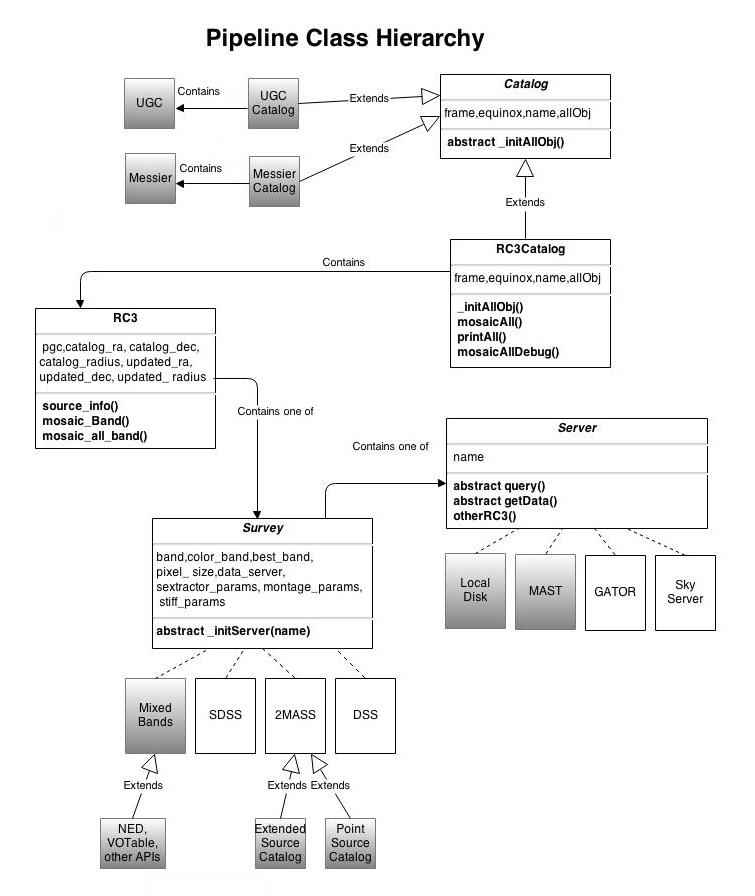
\includegraphics[width=0.5\textwidth]{pipeline}
		\caption{Greyed out boxes are possible extensions of this pipeline}
	\end{figure}
 	The motivation behind building a class hierarchy is to establish a mosaicking pipeline for any given catalog and survey data. We identify the essential components required for mosaicking program to work. The relationship between these essential steps are reflected in our design of the abstract $\texttt{Survey}$,$\texttt{Catalog}$, and $\texttt{Server}$ classes. 
 		\paragraph{Server}
		Data acquisition is composed of two main tasks: querying imaging data and retrieving data from server. Most surveys have an API that enables data access by SQL or customized query. Figure out how to convert positional values (ra,dec) to record-keeping parameters dependent on the survey's telescope. (tiles, frames...etc) For example, SDSS image frames are uniquely identified by a particular combination of  run,camcol,field.  Usually this step can be done using the SQL search. Our choice of using a server instead of a data object enables code reusability across various surveys that uses common server tools , such as IPAC's GATOR query service (\citet{irsa}) or  Astroquery.
	\paragraph{Catalog}
	The $\texttt{Catalog}$ class contains a list of objects that lies inside the catalog. Although the use of the Catalog container class seem unnecessary, it enables a clear separation between basic mosaicking functionality for individual galaxies. This can be used to study some particular object, executed on all objects in a $\texttt{Catalog}$, or simply used for debugging purposes. This abstraction barrier ensures minimal changes to the code in both classes when an investigator decides to input data from a new survey in the future.
\section{Result from SDSS run}
There are \_ RC3 galaxies within the footprint. 
on average the program processes 1.21 galaxies per minute
	\subsection{Known Errors}
	Even though a series of exception handling and error prevention mechanisms were put in place, 
	 	\begin{itemize}
	 		\item mProjectExec is the montage Mosaic procedure that creates the reprojected image from the raw FITS files. Sometimes reprojected images are not created even when Montages' debug statement clearly shows that the reprojection was successful and table and header files are corrupted. This results in an error in later mosaicing steps. We have implemented error prevention mechanism to ensure that mosaic procedures terminates correctly in such cases and wrote the problematic galaxy into failed\_projection, which can be examined later.
	 		\item Montage's background rectification module is not used in creating the FITS mosaics . Attempts were made in implementing these procedure, however it  is sometimes stuck in the step where the background model is applied to the projected images and  produces huge difference images files (\~50GB) for reason that we have not figured out yet. This should not affect the astrometric quality of the data product. The only visible diffference is observed in the color images for 2MASS, so will likely affect the photometric quality of the resulting 2MASS mosaics.(?)
	 	  \item DSS run lots of source confusion issue because it was never passed through the source confusion algorithm. 
	 		  %in coordir (\~)
	 	\end{itemize}
	
	\subsection{Performance}	
	\indent We accelerate the mosaicing process by performing the recursive algorithm on only a single band FITS file designated as $\texttt{best\_band}$, then mosacking all bands only once per object. For SDSS, we use the image obtained by the r band filter since transmission curve in \citet{edr} shows that r band has the highest quantum efficiency. 
	\\ \indent  Most of the computation time is spent on downloading the raw FITS files from the survey's specific server. Therefore, even though Montage's modular design enables its performance to scale with number of processor  (\citet{montage}), the process would not be significantly sped up by the use of Message Passing Interface (MPI). Therefore, the speed depends more on the bandwidth (downloading rate) rather than the number of cores in the machine. On <bigdog spec> machine, the program processes on average about 80 RC3 objects per hour using SDSS data. This average runtime would also depende on the sky coverage of the  particular survey , the speed of query ...etc . 
	\\ \indent This process can  be significantly sped up if the investigator already has imaging data stored locally on a disk or have access to running the mosaic program alongside the survey's datacenter. We have designed our class hierarchy such that this can be written as a subclass of $\texttt{Server}$ with user-defined details of where the images are stored.
The Montage 	mBgExec takes a long time . 

\section{Possible Uses of Data Product}
Can be incorporated in the photo pipeline in future survey to make pretty rc3 images.
with larger focal plane 
more photon
such as the LSST
saturation
especially with the DSS data, full coverage of the sky
map out where bright objects are. 


The scientifically calibrated FITS images can be used as for indivudual studies . It can be used for improved astrometry (as we did) in updating the catalog. Can also do photometry to determine galaxy property

Another possible usage is to combine the calibrated mosaics into multiband color images with mosaics from single/double band surveys such as POSS-I and GALEX.

 \section{Conclusion}
Can talk about here how LSST and future telescope can mask theses so that image not saturated
We provide data product for SDSS and DPOSS.
The FITS images can be used along with existing tools for scientific analysis on imaging data, such as Astrometry.net(\citet{astrometry.net}) , SExtractor, APLpy(\citet{aplpy}). We have provided documentation on GitHub \footnote{\url{https://github.com/ProfessorBrunner/rc3-sdss}} that guides investigators through the steps to adapting the pipeline for future imaging data. This can also be extended for other astronomical catalog such as the Messier Catalog or New General Catalog (NGC), as well as catalogs with user-defined selection limit. %user-defined catalogs used for (group, cluster,target??) studies. 

\section*{Acknowledgements}
\footnotesize
\indent We thank Harold G. Corwin, Jr. for helpful discussion that helped this work. This research made use of Montage, funded by the National Aeronautics and Space Administration's Earth Science Technology Office, Computation Technologies Project, under Cooperative Agreement Number NCC5-626 between NASA and the California Institute of Technology. Montage is maintained by the NASA/IPAC Infrared Science Archive. This research made use of Astropy, a community-developed core Python package for Astronomy (Astropy Collaboration, 2013).
\\
\indent  Funding for SDSS-III has been provided by the Alfred P. Sloan Foundation, the Participating Institutions, the National Science Foundation, and the U.S. Department of Energy Office of Science. The SDSS-III web site is http://www.sdss3.org/. SDSS-III is managed by the Astrophysical Research Consortium for the Participating Institutions of the SDSS-III Collaboration including the University of Arizona, the Brazilian Participation Group, Brookhaven National Laboratory, University of Cambridge, Carnegie Mellon University, University of Florida, the French Participation Group, the German Participation Group, Harvard University, the Instituto de Astrofisica de Canarias, the Michigan State/Notre Dame/JINA Participation Group, Johns Hopkins University, Lawrence Berkeley National Laboratory, Max Planck Institute for Astrophysics, Max Planck Institute for Extraterrestrial Physics, New Mexico State University, New York University, Ohio State University, Pennsylvania State University, University of Portsmouth, Princeton University, the Spanish Participation Group, University of Tokyo, University of Utah, Vanderbilt University, University of Virginia, University of Washington, and Yale University

\bibliography{bibtex_database}
 \bibliographystyle{abbrvnat}
\end{document}
